\section{Projected Gradient Descent}

PGD: do constrainted gradient descent. $y_{t+1} = x_t - \gamma \nabla f(x_t)$ then $x_{t+1} = \Pi_X(y_{t+1}) = \argmin_{X} \|x - y_{t+1}\|^2$.

\textbf{projection inequalities} (4.1): let $X$ be closed and convex, $x\in X$, then $(x - \Pi_X(y))^\top (y - \Pi_X(y)) \le 0$ and $\|x - \Pi_X(y)\|^2 + \|y - \Pi_X(y)\|^2 \le \|x - y\|^2$. Proof: $\Pi_X(y)$ minimizes $f(x) = \|x- y\|^2$ on $Z$, thus by optimality, $\nabla f(\Pi_X(y))^\top (x - \Pi_X(y)) = 2(\Pi_X(y) - y)^\top (x - \Pi_X(y)) \ge 0$ for any $x \in X$. The second follows from $2a^\top b = \|a\|^2 + \|b\|^2 - \|a - b\|^2$. Illustration:
    \begin{center}
        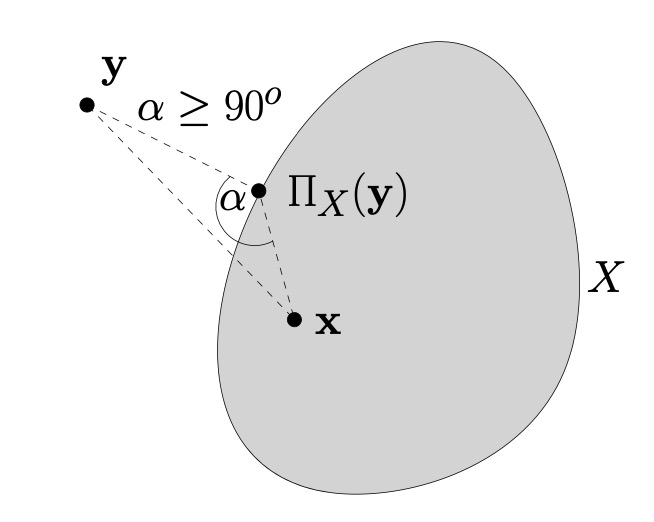
\includegraphics[width=.6\linewidth]{imgs/projection.jpg}
    \end{center}

\textbf{Analysis for PGD}: the same result but proof adapted using projection inequalities.
\begin{enumerate}
    \item Vanilla analysis: the same analysis for PGD gives $g_t^\top (x_t - x^*) = \frac{1}{2\gamma}\left(\gamma^2 \|g_t\|^2 + \|x_t - x^*\|^2 - \|y_{t+1}-x^*\|^2\right)$. By projection inequality, we have $\|x_{t+1} - x^*\|^2 \le \|y_{t+1} - x^*\|^2$. Thus, the result of vanilla analysis is the same.
    \item Lipschitz convex functions: (4.2) the same as GD since it only requires the result of vanilla analysis.
    \item $L$-smooth functions: (4.3) with $\gamma = 1/L$, we have $f(x_{t+1}) \le f(x_t) - \frac{1}{2L}\|\nabla f(x_t)\|^2 + \frac{L}{2}\|y_{t+1} - x_{t+1}\|^2$. In addition, $f(x_{t+1}) \le f(x_t)$. Proof: write the smoothness definition for $x_{t+1}$ for $x_t$. Replace $\nabla f(x_t)^\top (x_{t+1} - x_t)$ by $-L (y_{t+1} - x_t)^\top (x_{t+1} - x_t)$ and then apply $2a^\top b = \|a\|^2 + \|b\|^2 - \|a - b\|^2$ gives the first result. Since $\|y_{t+1} - x_{t+1}\| \le \|y_{t+1} - x_t\| = \gamma \|\nabla f(x_t)\|$, we have $f(x_{t+1}) \le f(x_t)$.
    \item Convex $L$-smooth functions: (4.4) the same result as GD. Proof: we use a tighter inequality for vanilla analysis. Instead of using $\|x_{t+1} - x^*\|^2 \le \|y_{t+1} - x^*\|^2$, we now use $\|x_{t+1} - x^*\|^2 + \|y_{t+1} - x_{t+1}\|^2 \le \|y_{t+1} - x^*\|^2$, so the vanilla analysis results in $\sum_{t=0}^{T-1} (f(x_t) - f(x^*)) \le \frac{1}{2L}\sum_{t=0}^{T-1} \|g_t\|^2 + \frac{L}{2}\|x_0 - x^*\|^2 - \frac{L}{2}\sum_{t=0}^{T-1} \|y_{t+1} - x_{t+1}\|^2$. Combining this with (4.3) gets the result.
    \item $\mu$-strongly convex and $L$-smooth functions: (4.5) PGD with $\gamma = 1/L$ yields $\|x_{t+1}-x^*\|^2 \le (1-\frac{\mu}{L})\|x_t - x^*\|^2$ and $f(x_T) - f(x^*) \le \frac{L}{2}(1-\frac{\mu}{L})^T \|x_0 -x^*\|^2 + (1-\frac{\mu}{L})^{T/2}\|\nabla f(x^*)\|\|x_0 - x^*\|$. This is still $O(\log(\frac{1}{\epsilon}))$ steps. Proof: $\mu$-strongly convexity strengthens the vanilla analysis to be $g_t^\top (x_t - x^*) \le \frac{1}{2\gamma}(\gamma^2 \|g_t\|^2 + \|x_t - x^*\|^2 - \|x_{t+1}-x^*\|^2 - \|y_{t+1} - x_{t+1}\|^2) - \frac{\mu}{2}\|x_t - x^*\|^2$. This makes the vanilla analysis to give $\|x_{t+1}-x^*\|^2 \le 2\gamma \left(f(x^*) - f(x_t)\right) + \gamma^2 \|\nabla f(x_t)\|^2 + (1-\mu\gamma)\|x_t - x^*\|^2 - \|y_{t+1} - x_{t+1}\|^2$. The extra $- \|y_{t+1} - x_{t+1}\|^2$ happens to compensate for the additional term from the $L$-smoothness, thus (i) follows. By smoothness, we have $f(x_T) - f(x^*) \le \|\nabla f(x^*)\| \|x_T - x^*\| + \frac{L}{2} \|x_T - x^*\|^2$, thus (ii) follows from (i).
\end{enumerate}

\textbf{Projecting into $L_1$ ball}: solve $\Pi_X(v) = \argmin_{\|x\|\le 1}\|x-v\|^2$. WLOG, assume $v_1 \ge v_2 \ge \dots v_d \ge 0$ and $\sum_i v_i > 1$. (4.11) We have $x_i^* = v_i - \theta_p$ for $i\le p$ and $x^*=0$ for $i>p$, where $\theta_p = \frac{1}{p}(\sum_{i=1}^p v_i -1)$ and $p=\max\{p \in [d]: v_p - \frac{1}{p}(\sum_{i=1}^p v_i - 1)>0\}$. This makes the projection $O(dlog d)$. Actually it can be improved to $O(d)$.